
% !TeX spellcheck = en_US

\chapter{Introduction to Flyway}


\section{Overview}
\marginpar{Information}%
Flyway is a tool that makes database migrations easy and provides version control for your database. It is a multi-platform and cross-database tool with support for over 20 databases.
Axel Fontaine from Google Code created Flyway in 2010, and acquired by Redgate Software by 2019. Flyway is currently at the 9th version when creating this work. The creator was looking for a simple method to implement database changes easily and directly in SQL. His main goal was, to include database changes as part of the software deployment process \cite{Robles2021}.
Flyway uses the freemium business model.  The basic version is free and open source \cite{Fontaine2010} and additionally there is a paid Teams or Enterprise Edition available.\\
With flyway you can either write migration files with SQL (database-specific syntax (such as PL/SQL, T-SQL, etc.) or Java (for advanced data transformations or dealing with LOBs). Flyway is able to connect to databases hosted in either on-premises or cloud environments, thanks to the included JDBC driver library that is shipped with the tool. It runs on all modern platforms such as Linux, Mac or Windows.  \cite{Dillon2022}, \cite{DBMSTools}


\marginpar{Migrations \cite{Parsick2018}}%
There are four possibilities of migrations as shown in \autoref{tab:migration_types}. There are versioned migrations with scripts that have a unique meaning, which are executed only once. These versioned migrations are mainly used for Data Definition Language (DDL) like a create or modify a table. \\

Repeatable migration scripts do not have a version number. These are always if their checksum changes and always after the versioned migrations are applied. Typical applications are import base data or (re)-create views or functions.

\begin{table}[h]
	\centering
	\begin{tabularx}{8cm}{X|c c}
		& Versioned & Repeatable \\ \hline
		SQL based & \checkmark & \checkmark \\
		Java based & \checkmark & \checkmark \\
	\end{tabularx}
	\caption{Migration Types - Based on \cite{Parsick2018}}
	\label{tab:migration_types}
\end{table}

%\begin{center}
%\begin{tabularx}{8cm}{X|c c}
%	& Versioned & Repeatable \\ \hline
%SQL based & \checkmark & \checkmark \\
%Java based & \checkmark & \checkmark \\
%\end{tabularx}
%\end{center}


\marginpar{SQL migrations}%
Flyway developers can migrate changes directly with SQL. Per default, flyway takes the database migrations from the directory \textit{sql}.
These SQL migration files have to follow the naming convention:\\

\begin{center}
\begin{tabularx}{8cm}{r l}
Versioned & \texttt{\textcolor{blue}{V}\textcolor{green}{1\_1\_1}\textcolor{red}{\_\_}\textcolor{orange}{create\_table}.sql}\\
Repeatable & \texttt{\textcolor{blue}{R}\textcolor{red}{\_\_}\textcolor{orange}{create\_table}.sql}\\
\end{tabularx}
\end{center}

\begin{flushright}
\textcolor{blue}{Prefix}\\
\textcolor{green}{Version}\\
\textcolor{red}{Seperator (two underscores)}\\
\textcolor{orange}{Description}\\
\end{flushright}

These SQL scripts can have several rows and allowed is all database specific syntax including comments. These SQL migrations are mainly used for DDL changes such as create, alter, drop, etc. or for simple data changes.

\marginpar{Java migrations}%
Unlike changes in SQL, changes in java are more for BLOB or CLOB changes or for advanced changes to a large data set like recalculations. The naming convention is pretty similar, only the ending differs.\\
\begin{center}
	\begin{tabularx}{8cm}{r l}
		Versioned & \texttt{\textcolor{blue}{V}\textcolor{green}{1\_1\_1}\textcolor{red}{\_\_}\textcolor{orange}{create\_table}.java}\\
		Repeatable & \texttt{\textcolor{blue}{R}\textcolor{red}{\_\_}\textcolor{orange}{create\_table}.java}\\
	\end{tabularx}
\end{center}

\marginpar{Advanced changes\\ \cite{Parsick2018}}%
Sometimes you have to intervene between certan migration steps. For example, when creating a materialized view. This functionality is provided by flyway with callback functions. 


\begin{figure}[H]
	\centering
	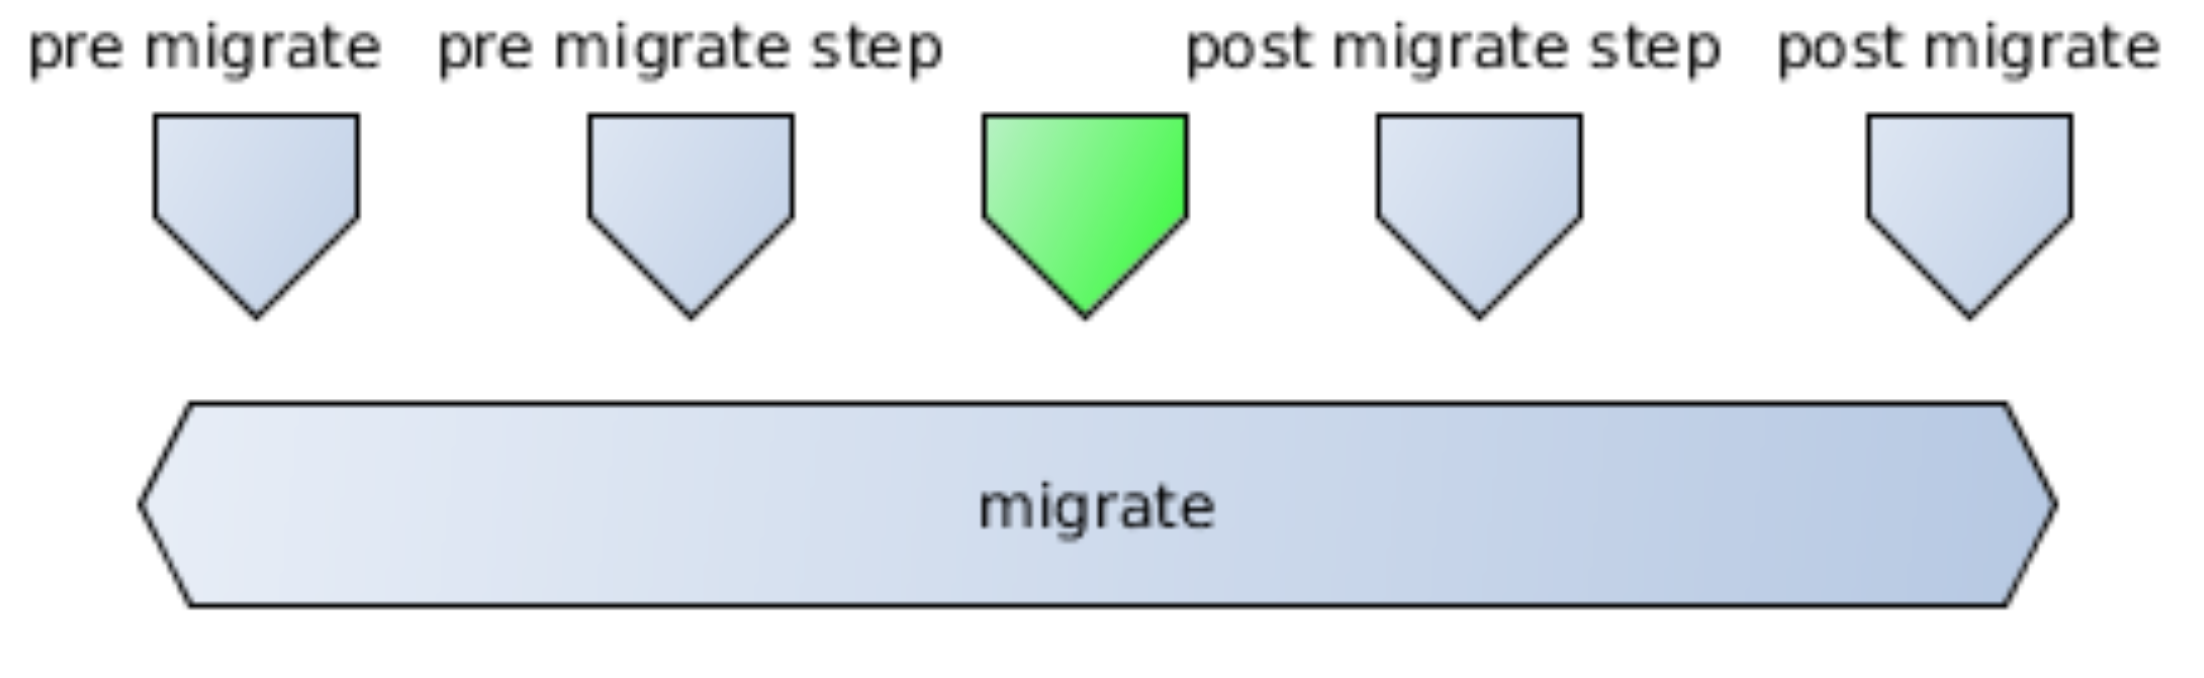
\includegraphics[width=0.6\textwidth]{./chapters/intro_flyway/images/advanced_migrations}
	\caption[Flyway Lifecycle - Source: \cite{Parsick2018}]{Flyway Lifecycle}
	\label{fig:advanced_migrations}
\end{figure}

There are several options for the execution times. These times are recognized with the help of the names. One can either write this callbacks in SQL or in Java. 

\begin{lstlisting}[caption=SQL Callback Functions for Flyway - Source: \cite{FlywayCallbacks}]
BeforeMigrate.sql
BeforeEachMigrate.sql
AfterEachMigrate.sql
AfterMigrate.sql
\end{lstlisting}

If the task needs to be more powerful or flexible, Java callbacks can be formulated as following:
\begin{lstlisting}[caption=Java Callback Functions before clean - Source: \cite{FlywayCallbacks}]
public interface FlywayCallback {

	/**
	* Runs before the tasks executes
	* by avoiding unnecessary connection state setups for events that will not be handled anyway.
	*
	* @param valid connection to a database
	*/
	void beforeClean(Connection connection);
	
}
\end{lstlisting}
Other callback function can be formulated with the same name as the SQL-functions.

\marginpar{Features}%
\todo{Soll das Folgende in den Anhang?}

In the following paragraph, a few very useful flyway commands are presented:\\

\textbf{Info}\\
Get an overview of the applied migrations and their success status.\\

\begin{figure}[H]
	\centering
	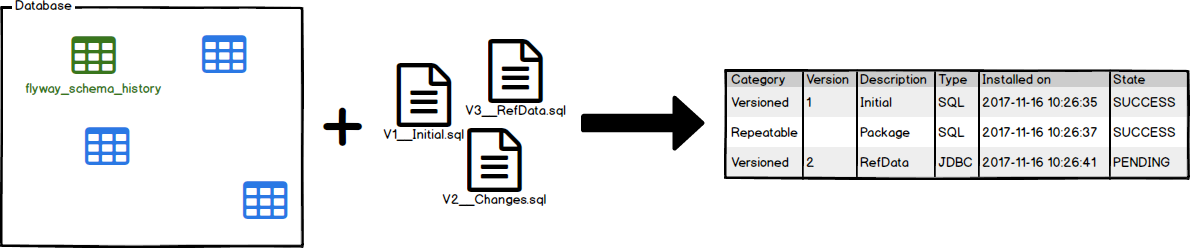
\includegraphics[width=0.4\textwidth]{./chapters/intro_flyway/images/command-info}
	\caption[Flyway Info - Source: \cite{FlywayGetStarted}]{Flyway Info}
	\label{fig:command-info}
\end{figure}


\textbf{clean}\\
With \texttt{flyway clean} one can drop all objects like tables, views, triggers, etc. in the configures schemas.It can easily give you a fresh start but is dangerous in a production environment.

\textbf{Validate}\\
If one want to be sure that all migrations are applied correctly,  \texttt{flyway validate} is the command of choice. The validation checks if the migration locally still has the same checksum as the migration executed in the database.
There is a possibility to apply custom validation rules. Because in a productive environment, there will be hotfixes, deleted migrations and other changes that break the default validation conventions (Flyway Teams Edition only).

\textbf{Repair}\\
But if something is broken, you can use this command to repair the database and especially the checksum. When a database migration fails, the migration is markes as failed in the schema history table (\textit{flyway\_schema\_history}). If a database supports DDL \footnote{Data Definition Language} transactions (like PostgreSQL), the failed migration is rolled back automatically and nothing is recorded in the schema history table.  But if the database does not support DDL transactions (e.g. Oracle Database, MySQL, MariaDB), you have two options to repair the database and remove the failed entries:

\begin{enumerate}
	\item Run \texttt{flyway repair}\\
	\item One uses the flyway callback functions. One could use the \textit{afterMigrateError} and add a SQL-script to this callback, which deletes the failed migration entry in the \textit{flyway\_schema\_history} table.
	
	\begin{lstlisting}[language=SQL]
		DELETE IGNORE FROM flyway_schema_history WHERE success=0;
	\end{lstlisting}
\end{enumerate}


\textbf{Undo}\\
To undo the most recent migration applied to the database, run \texttt{flyway undo}. The undo command can be repeated until the database is converted back to version 1.
Undo assumes that the previous applied migration succeeded and now should be undone. If the previsous applied migration failed, first repair the migrations before applying the undo-command. 
The undo-command is a Teams Edition feature only.

\textbf{Baseline}\\
This command makes the current database as the baseline for the future. This will cause Migrate to ignore all migration up to the actual version.
This can be useful to reduce the overhead, if you have many old migrations scripts that will not be used anymore.

\marginpar{Flyway Teams \cite{FlywayTeams}}%
The Pro-Version of Flyway is called Flyway Teams. This pro version costs (as of creation of this work) 447€ per user per year. It offers:
\begin{itemize}
	\item Additional migration controls
	\item Protect against failed deployments
	\item Professional echnical support from Redgate
	\item Support for older DB versions
	\item Built-in Git client and object-level versioning
\end{itemize}

In comparison to the team version, the free open source version includes the core functionalities with a Desktop GUI support for only the current DB versions and support through community. The core functionalities include the six basic commands: Migrate, Clean, Info, Validate, Baseline and Repair.\\

A comparison between the Flyway editions can be found here \autoref{label}.\\
\todo{Liste einfügen in Anhang}

\marginpar{Community}%
Stars on GitHub: 6'800 (31. October 2022)\\
Tags in StackOverflow: 2,088 (31. October 2022)\\

\marginpar{Learning\\ Materials}%
If you have never worked with Flyway before there are the following ways to educate yourself:
\begin{itemize}
	\item \href{https://www.red-gate.com/hub/university/courses/flyway}{Redgate University Flyway training courses}
	\item \href{https://flywaydb.org/documentation}{Get Started Documentation}
	\item \href{https://www.youtube.com/playlist?list=PLhFdCK734P8DYHYYWaJpzJJ-qZFZ_JTHM}{Redgate Youtube Channel}
	\item \href{https://www.youtube.com/watch?v=dzRzlDpdDW4}{Flyway talk by Sandra Parsick}
\end{itemize}

\section{Installation and Setup}
\marginpar{Different usages of Flyway}%
\todo{https://flywaydb.org/documentation/usage/plugins/}

\marginpar{CLI installation}%
Download the latest version of the \href{https://flywaydb.org/download/community}{Flyway Cummunity Edition} and extract the downloaded file. To execute the flyway commands, one need a java installation.
Once extracted, the file becomes a directory with the following structure:

\begin{figure}[H]
    \centering
    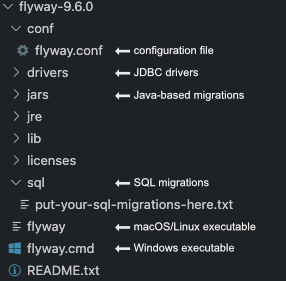
\includegraphics[width=0.4\textwidth]{./chapters/intro_flyway/images/flyway_folder_structure}
   \caption[Flyway folder structure - Source: Own illustration]{Flyway folder structure}
    \label{fig:flyway_folder_structure}
\end{figure}


\marginpar{Configuration}%
To connect to a running database, add the relevant information to \textit{conf/flyway.conf}.
In our minimal example this could be:

\begin{lstlisting}[caption=Minimal configuration]
flyway.url=jdbc:postgresql://localhost:5432/pagila
flyway.user=postgres
flyway.password=password
\end{lstlisting}

This is just a minimal configuration, but there are many more additional parameters that can be set \footnote{\url{https://flywaydb.org/documentation/configuration/parameters/}}.


\marginpar{Workaround Mac OS}%
To make the flayway command know on MacOS:
\begin{lstlisting}[caption=Minimal configuration]
export PATH=$PATH:/Users/marco/Documents/DB-Seminar/flyway-9.8.1
\end{lstlisting}
Running a flyway command for the first time, the error message \textit{„java“ kann nicht geöffnet werden, da der Entwickler nicht verifiziert werden kann.} occurs. Go to Security in settings and allow the java instance to run.

\newpage